\chapter{The role of \textit{Cis}-Regulatory elements in \textit{Astyanax mexicanus} morphological adaptation to cave environment}
\label{sec:cap_astyanax}


In the first part of the project, we investigated changes in gene regulation at relatively large evolutionary distances. We demonstrated a regulatory rewiring of the main developmental signalling pathways in the transition from chordate invertebrates to vertebrates. However, evolution and gene regulation can also operate at the microevolutionary scale. In this chapter, we aim to unravel the role of gene regulation in adaptation to a new environment. To understand microevolutionary changes in gene regulation, we used \textit{Astyanax mexicanus} as a model organism. The cavefish population of this species has undergone striking phenotypical adaptations to the cave, like lack of pigmentation, complete degeneration of the eye, several metabolic adaptations and enhanced mechanosensory organs, together with behavioural changes. We performed ATAC-seq and RNA-seq experiments in both morphotypes of \textit{Astyanax}, the cavefish (\textit{Pachón} population) and the surfacefish in different developmental stages. Then, we analysed these datasets in order to get insight into the regulatory differences underlying the adaptation to the cave environment. We also generated a set of genomic alignments using the Cactus pipeline \parencite{armstrong_progressive_2020} to study the evolutionary history of the regulatory changes.


\section{Comparing the development of Surfacefish and Cavefish at epigenetic and transcriptomic level}

First, we analyzed the ATAC-seq data at different developmental stages in \textit{Astyanax mexicanus}. These stages were 80\% of epiboly, 5 somites (5ss), 24hpf and 48hpf. We could identify several thousands of open chromatin regions in each stage of the cavefish and surfacefish development, and then we performed differential analysis between cavefish and surfacefish equivalent stages using DESeq2 \parencite{love_moderated_2014} as the statistical framework. Then, to gain insight into the biological functions of the DARs found and TFs binding onto them, we clustered the ATAC-seq signal of these DARs according to their developmental stage. Using the Homer toolkit for TFBS enrichment, we assessed which TFBS prevail in each cluster of DARs (Figure \ref{fig:ast_dar_clustering}). We found several TFs enriched in these clusters of differentially accessible regions between the two morphotypes, with several of them known to be related to cave adaptation mechanisms. For example, the \textit{klf} transcription factor family was consistently enriched between the two populations at any given stage. These factors are implicated in several developmental functions \parencite{antin_embryonic_2010} important for adaptation to cave environments, like retinal development \parencite{gautam_multi-species_2021} or metabolism regulation\parencite{li_kruppel-like_2022}. Moreover, we were able to detect TFs related to different cavefish phenotypes, such as \textit{hnf4a}, which is important for insulin resistance \parencite{warren_chromosome-level_2021, krishnan_genome-wide_2022}. We investigated the genes nearby each set of DARs, associating each DAR with target genes. We performed GO enrichment analysis for these genes, and we found that they were related to cave adaptation processes such as pigmentation, metabolism, and circadian rhythm.


\begin{figure}
\centering
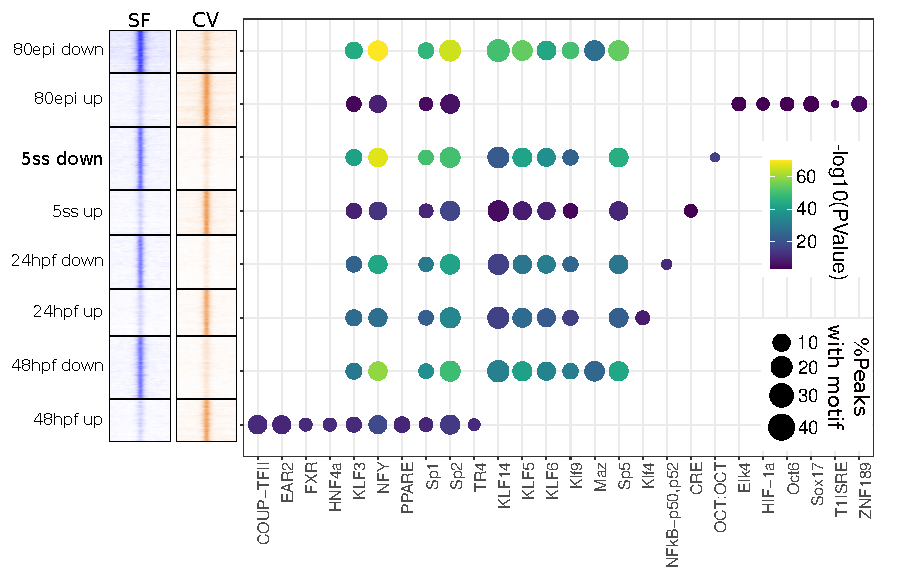
\includegraphics[width=1\textwidth]{Figures/astyanax/DAR_clustering}
\caption[Clustering of DARs between surfacefish and cavefish]{Clustering of ATAC-seq signal in DARs between surfacefish and cavefish. On the left of the panel, the clustering of the ATAC-seq signal in DARs is represented for each group in surfacefish (SF, blue colour) and cavefish (CV, orange colour). On the right, a dot plot of the top 10 TFBS most enriched for each of the groups. The Y-axis corresponds to the DARs groups, which are aligned in the heatmap with the dot plot. TFBS names are represented in the X-axis. The size of the dots is proportional to the \% of peaks in the DAR group that contains this specific TFBS. The colour of the dots represents the $-log10(PValue)$ of the enrichment. We can observe that there is a great level of overlapping in the enrichment of TFBS, with some TFBS enriched only in more specific clusters.}
\label{fig:ast_dar_clustering}
\end{figure}


To gain insight into the transcriptomic changes induced by the differential regulation, we performed clustering analysis of RNA-seq profiles by grouping genes according to their differential expression (Figure \ref{fig:ast_gene_clustering}). We then computed the GO enrichment for these groups of genes and found a large number of processes relevant to cave adaptation in accordance with the ATAC-seq analysis. In fact, we detected altered developmental and metabolic processes, which are common in troglomorphic traits. Interestingly, we also observed that visual perception is a process enriched in the group of genes that were downregulated at the 24 hpf stage. Indeed, this is roughly the time when the lens starts to degenerate in cavefish populations, ultimately leading to the degeneration of the entire eye \parencite{jeffery_regressive_2009, ma_hypomorphic_2020, strickler_lens_2007}. Taken together, the previous transcriptomic and epigenomic data, we are confident to speculate that there are important variations in the GRN of eye specification between the two morphotypes.


\begin{figure}[hp]
\centering
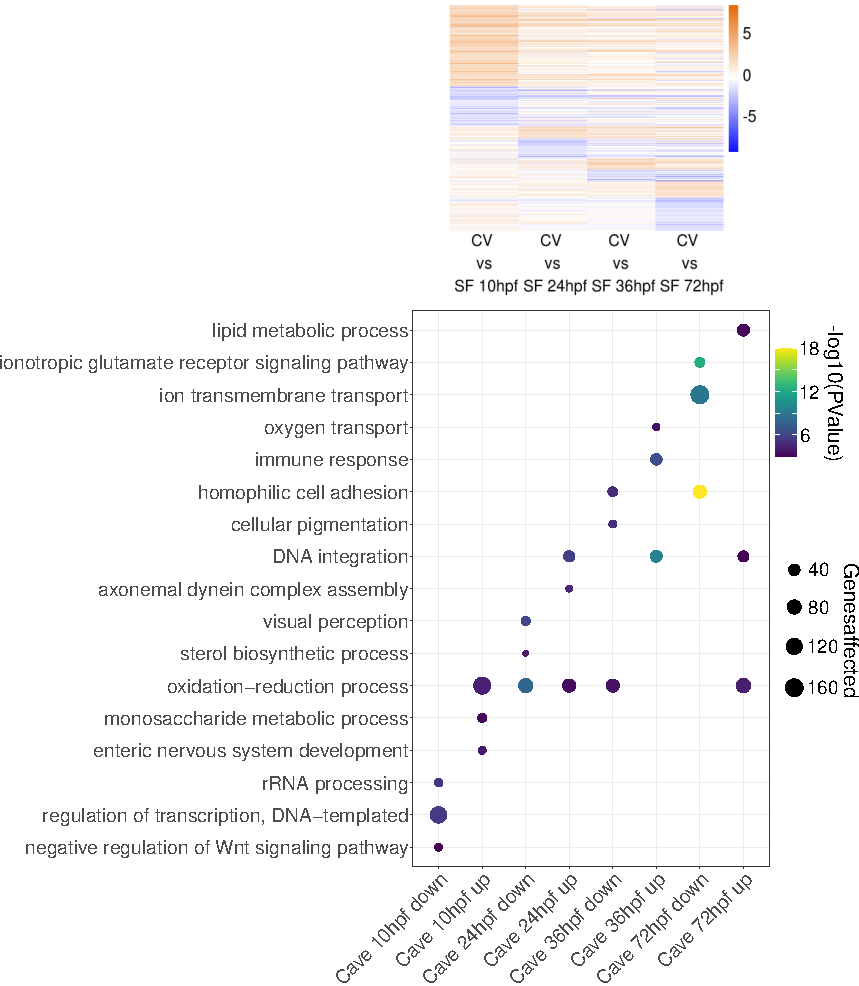
\includegraphics[width=1\textwidth]{Figures/astyanax/Diff_genes_clustering}
\caption[Clustering of genes between surfacefish and Cavefish]{Clustering of differential genes detected by RNA-seq and their associated GO term enrichment. On the top panel, the different clusters of genes are represented based on their $log2(FC)$. Upregulated and downregulated genes are represented in orange and blue, respectively. Each comparison is represented in the X-axis. The bottom panel represents the GO enrichment. X-axis represents each group of differential genes. Y-axis represents the enriched GO terms. Dot size is proportional to the number of genes enriched in that GO term. The colour of the dots varies with the $-log10(PValue)$ of the enrichment.}
\label{fig:ast_gene_clustering}
\end{figure}

Next, we focused on differentially regulated genes that are also associated with DARs, the DSGs (Double Selected Genes), as determined previously. In the previous chapter, we demonstrated that DSGs are enriched in core genes of changing GRNs. In this case, this analysis allowed us to narrow down the genes that contributed to the adaptation to the cave environment. Here, we focused only on the DSGs at 24hpf due to the lack of available paired-in-time ATAC-seq and RNA-seq data of other developmental stages. In total, we identified 1138 DSGs at 24hpf, which were regulated by 2061 DARs. To explore the functions of these genes, we computed GO term enrichment in this set of DSGs. As indicated from the previous analyses, we found processes highly related to cave adaptation, such as lipid metabolism, melanosome organisation (pigmentation development), visual perception, or whole organism development. More precisely, these functions involve developmental genes like \textit{otx2a} or \textit{vax2} genes, which are implicated in eye development \parencite{martinez-morales_otx2_2003, buono_analysis_2021}. To gain a better understanding on the regulation of these DSGs, we looked into the DARs regions that were associated with DSGs to detect the TFs that preferentially regulate these sets of core genes. This analysis revealed many TFs implicated in regulating DSGs at the 24hpf stage. While some of them, such as the \textit{klf} TF family, appeared already in the equivalent analysis based only on DARs, we could find some additional ones. For instance, calcium response elements, known to be important in the cave adaptation process via eye degeneration \parencite{keene_biology_2015}, were highly enriched. Moreover, we also detected TFBS enrichment of main circadian rhythm components like the \textit{clock} TF. It has been shown that cavefish have their circadian rhythm and associated behaviour altered due to changes in the expression of regulators of this process \parencite{beale_circadian_2013, olsen_circadian_2023}.





%\begin{figure}
%\centering
%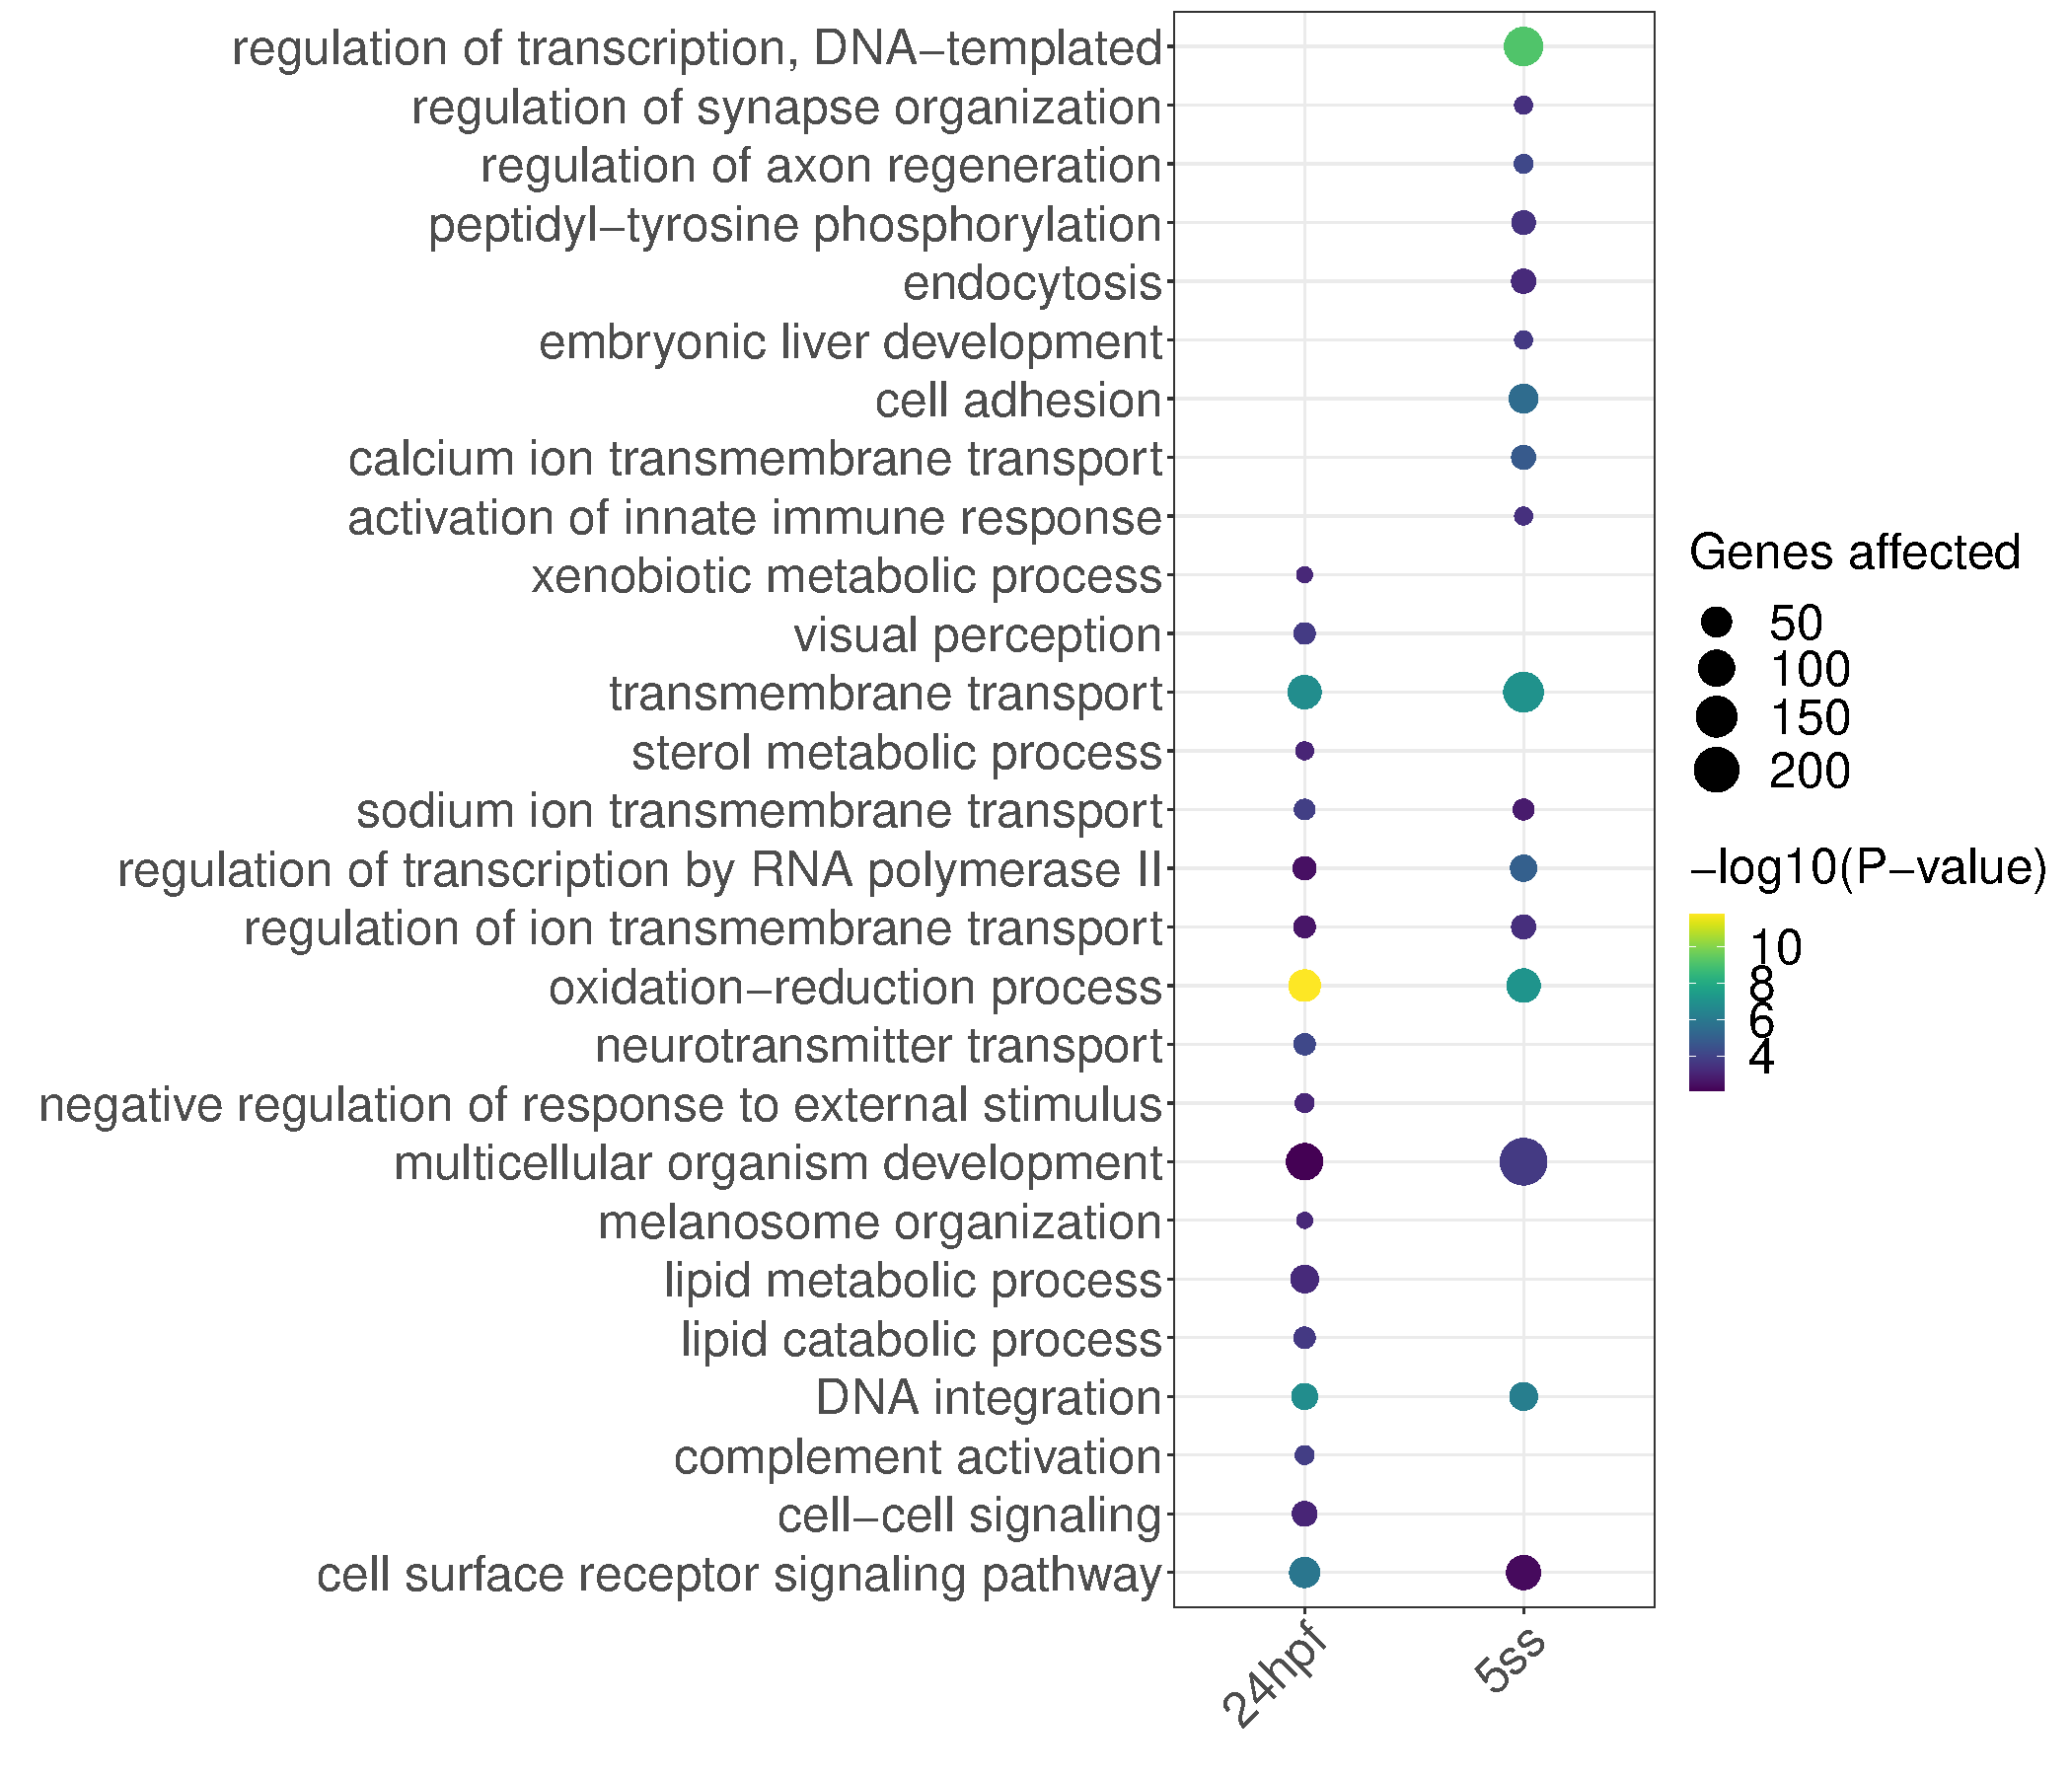
\includegraphics[width=1\textwidth]{Figures/astyanax/GO_DSG}
%\caption[Astyanax DSGs revealed key processes to cave adaptation]{Astyanax DSGs revealed key processes to cave adaptation}
%\label{fig:astmex_dsg_analysis_GO}
%\end{figure}


%\begin{figure}
%\centering
%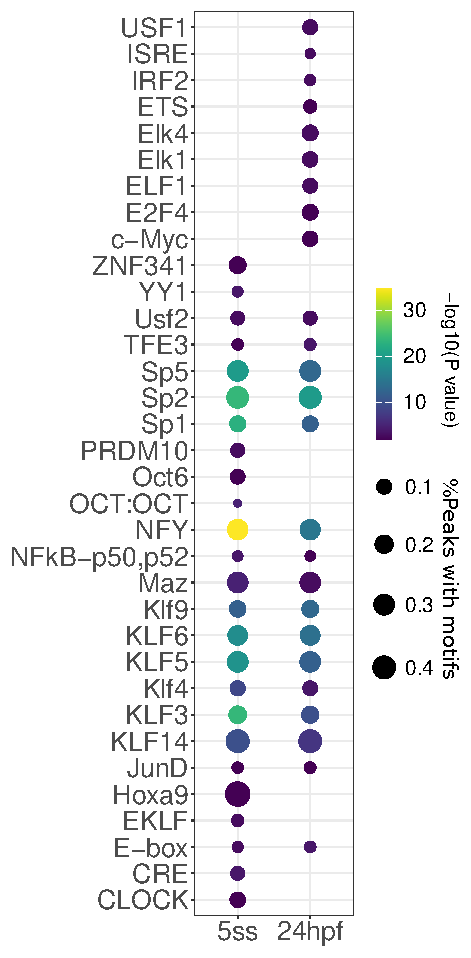
\includegraphics{Figures/astyanax/TFBS_DSG}
%\caption[Astyanax DSGs TFBS enrichment]{Astyanax DSGs revealed key TFs to cave adaptation}
%\label{fig:astmex_dsg_analysis_TFBS}
%\end{figure}

\begin{figure}[hp!]
\centering
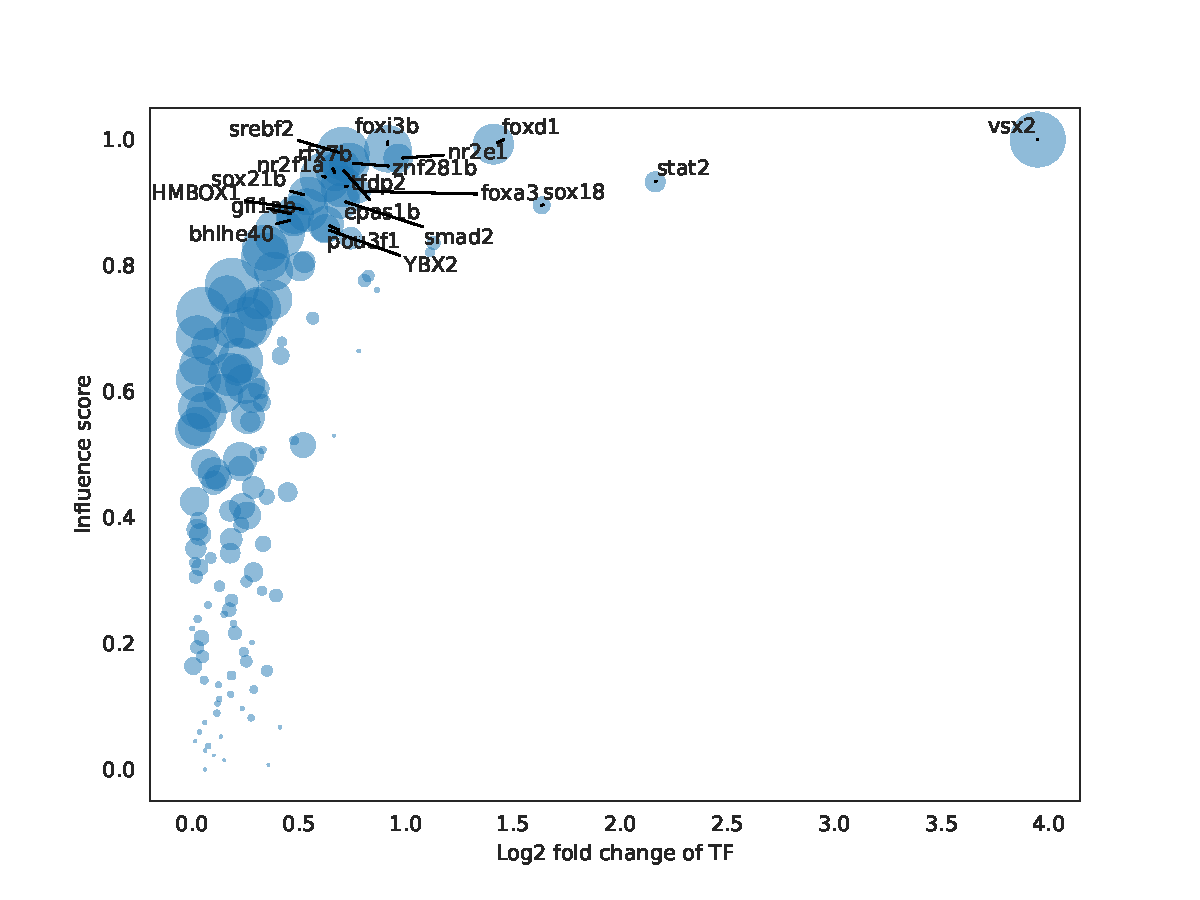
\includegraphics[width=1\textwidth]{Figures/astyanax/influence_plot_24hpf_cave_2_surface}
\caption[ANANSE influence plot]{Dot plot representing the influence score of TFs. RNA-seq expression $log2(FC)$ of each TF is represented in the X-axis. Influence score, which ranges from 0 to 1, is represented in the Y-axis. The top 20 most influential TFs are named. The size of the dots is proportional to the number of genes regulated by these TFs.}
\label{fig:Ananse_networks_plot}
\end{figure}


The DSG analysis highlighted that several processes were simultaneously altered in cavefish in the course of the adaptation to the cave environment. It is then plausible to suggest that key developmental GRNs are altered in this process and the findings of our analyses confirmed the involvement of known effector genes of these GRNs. To elucidate and visualize better the GRNs changes that took place, we used ANANSE \parencite{xu_ananse_2021}, which integrates ATAC-seq and RNA-seq information (see \ref{sec:integration_atac_rna} for more technical details). Originally this algorithm was designed to decipher the GRN changes that drive the differentiation of one cell type to another unidirectionally. The algorithm computes an "influence" score, which measures the importance of a given TF is for this differentiation \parencite{xu_ananse_2021}. In this work, we used this algorithm to reveal the most influential TFs for the adaptation of \textit{Astyanax mexicanus} to the cave environment. We computed differential GRNs for the 24hpf stage, in which we have paired ATAC and RNA-seq information (Figure \ref{fig:Ananse_networks_plot}). The analysis of this network revealed that several TFs explained most of the differences between surfacefish and cavefish GRNs. Some of them belonged to the eye developmental GRN, like \textit{vsx2} or \textit{bhlhe40} (Figure \ref{fig:Ananse_networks_network}). We also found TFs related to muscle development, like \textit{myod} and \textit{myog} genes, or to the metabolic adaptations to the cave environment, like \textit{klf11b} or the aforementioned TF \textit{hnf4a}, reflecting the role that these GRNs have in cavefish adaptation. These results, together with the previous analyses performed, underscore some of the main TFs driving the regulatory adaptation to the cave environment.





\begin{figure}[hp!]
\centering
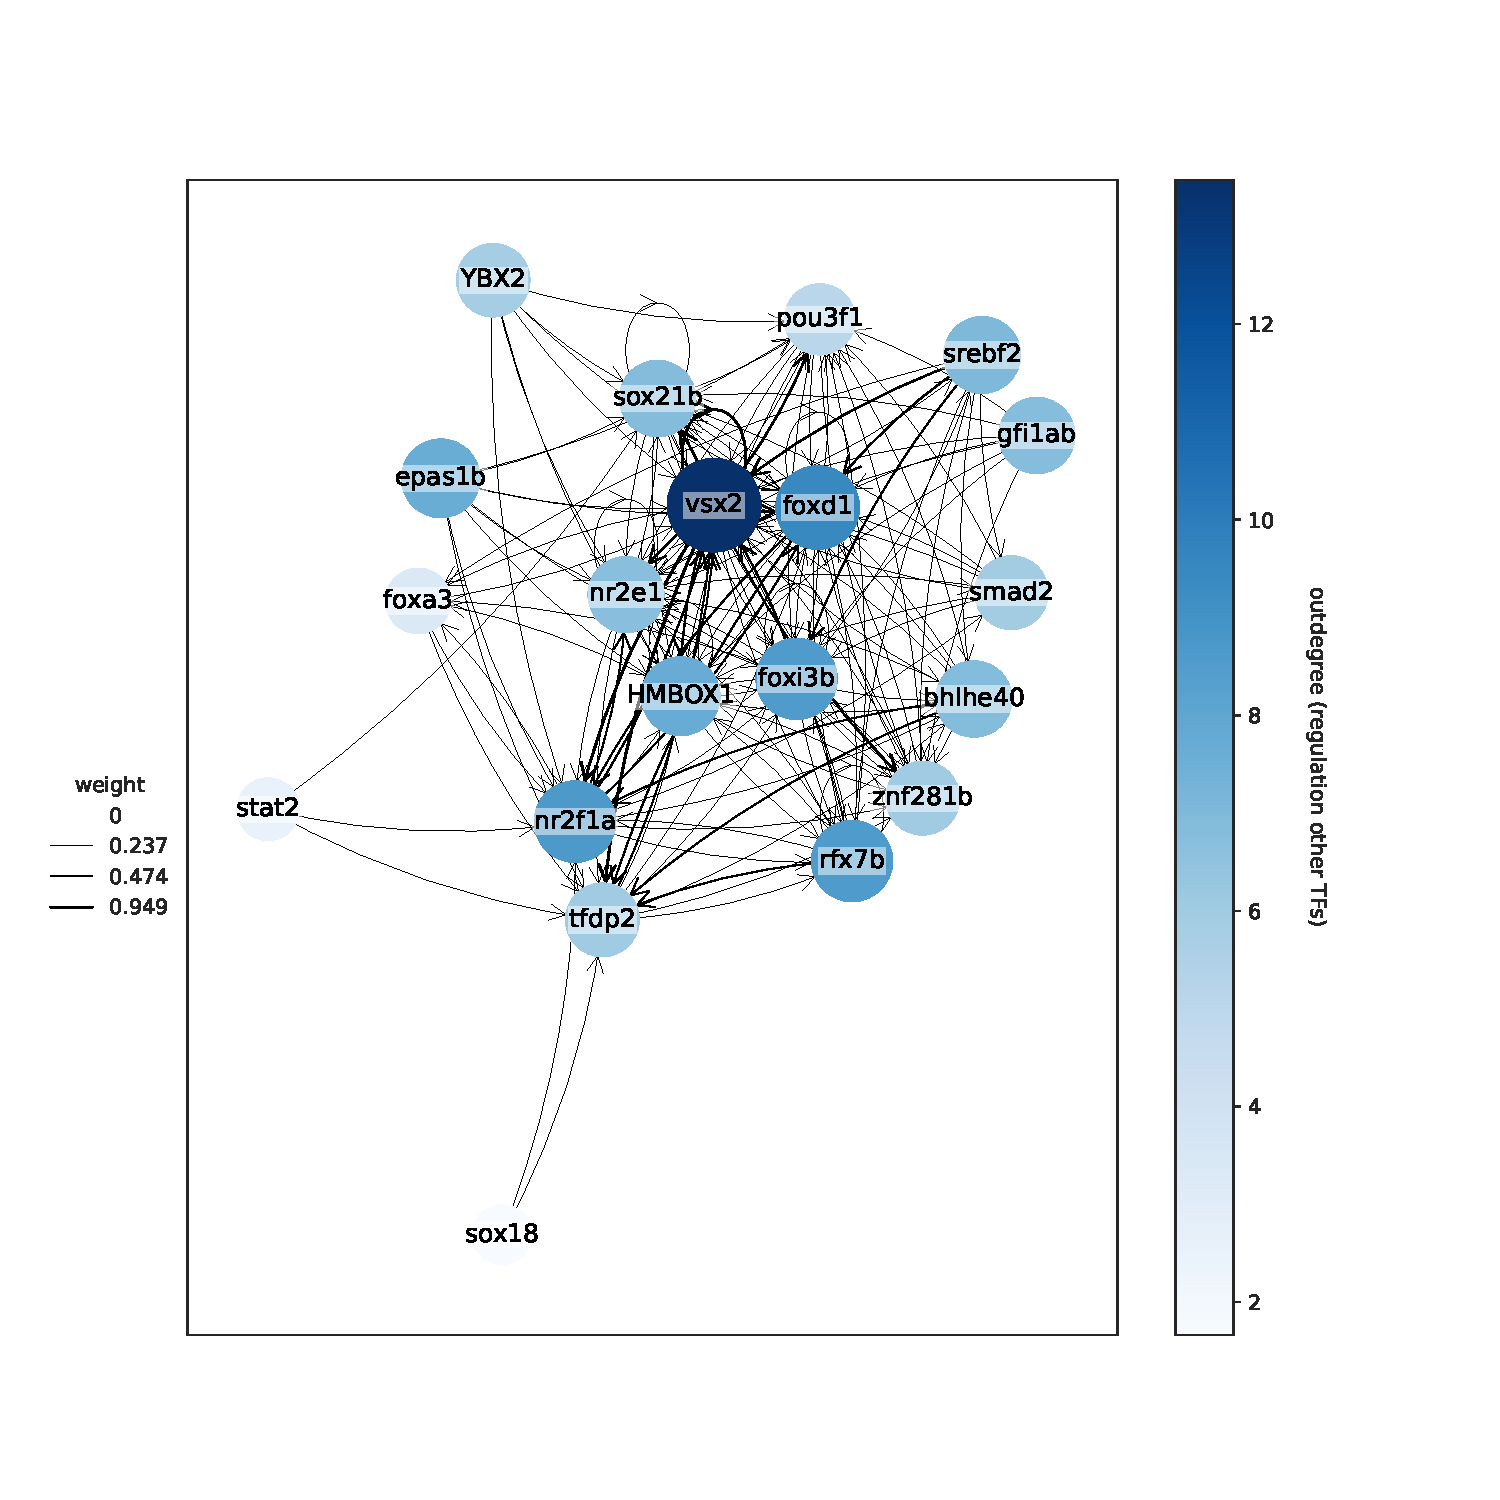
\includegraphics[width=1\textwidth]{Figures/astyanax/topTF_GRN_24hpf_cave2surface}
\caption[ANANSE networks]{Representation of the differential GRN between cavefish and surfacefish. In this representation, the most influential TFs are arranged in a network. The nodes of this network are the TFs themselves, and the arrows represent their interactions with other TFs. The colour of the nodes is proportional to the number of target genes regulated by the TFs.}
\label{fig:Ananse_networks_network}
\end{figure}




\section{Evolution of CREs at a micro-evolutionary scale}

Using ANANSE, we revealed interesting changes in the GRNs due to differential binding and activity of certain influential TFs. To better understand the underlying cause of the differential activity of TFs in the regulatory regions, we aimed to investigate the changes in CREs following two different approaches. 


First, applying CRISP software \parencite{bansal_statistical_2010} on our ATAC-seq data, we detected sequencing reads with a single nucleotide change in cavefish compared to surfacefish. The resulting variants were then intersected with the DARs obtained from comparing cavefish and surfacefish populations, resulting in 144 DARs with at least one single nucleotide variation. We then used TOBIAS and motifBreakR tools \parencite{bentsen_atac-seq_2020, coetzee_motifbreakr_2015} to assess the potential effect of these variations on TF binding ability. TOBIAS is a tool that infers the binding of TFs on TFBS by analysing the ATAC-seq signal footprint that TFs leave when they are bound to the genome, protecting their binding sites from Tn5 transposition. Motifbreakr allows us to analyze the effects of mutations in TFBS. This tool predicts how disruptive a variant is, taking into account the DNA preference of TFs. Together, we interrogated which single nucleotide variants within TFBSs impaired the binding of the TF in cavefish. Once we had the most affected TFBSs, we ranked them according to the number of times that these TFBSs had been affected. We found that the most changed TFBSs that significantly altered the binding of the corresponding TF were indeed identified in our previous analyses, such as \textit{klf} factors (Figure \ref{fig:Motifbreakr_tobias}). These results indicate that these TFs undergo changes in gene expression and also suffer disruption in their binding to target genes due to changes in the CREs, altering the expression of downstream target genes.


\begin{figure}
\centering
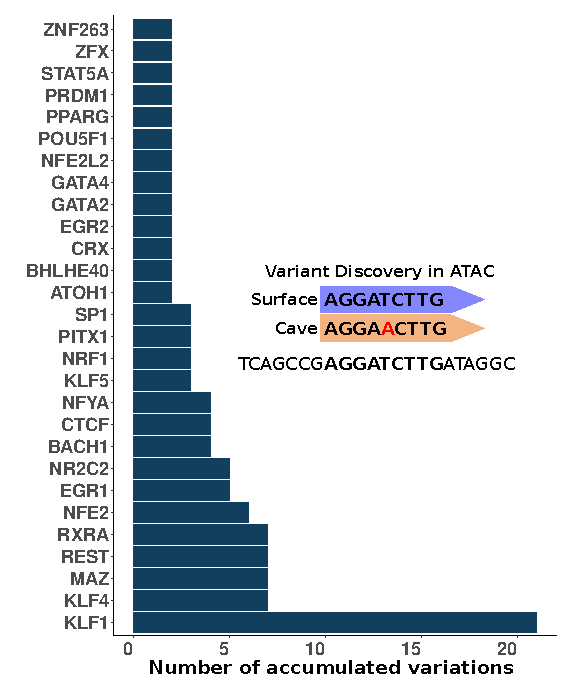
\includegraphics[width=1\textwidth]{Figures/astyanax/motifbrakr_tobias_results}
\caption[Motifbreakr and Tobias results]{Barplot representing the number of TFBS affected by nucleotide variations. A schematic representation of how variants were detected using ATAC-seq data is at the centre of the figure. Barplots represent the number of sites that are mutated and are altering TF binding. The TFs are ordered by the total number of their TFBSs that are altered.}
\label{fig:Motifbreakr_tobias}
\end{figure}


Next, using comparative genomics and the Cactus pipeline \parencite{armstrong_progressive_2020}, we obtained a suitable genomic alignment that included both morphotypes of \textit{Astyanax mexicanus} and phylogenetically close species of teleosts (for more details about this alignment, please see \ref{sec:comp_genomics}). Then, we computed the conservation score of CREs in \textit{Astyanax mexicanus} compared to the other teleost species. Regions that changed at an unexpectedly high rate were designated as accelerated regions (ARs). These regions accumulated more changes than expected, considering a neutral model of evolution. 

We computed the ARs of cavefish against all the other species in our analysis. These ARs are those regions of the genome that have changed the most in cavefish compared to the other assemblies of the alignment, including other species and surfacefish. The genomic positions of these regions were mostly non-coding regions, potentially affecting gene regulation rather than the gene products themselves \parencite{leclercq_evolution_2022}. Furthermore, we investigated which regulatory information these ARs were encoding. To do this, we computed the enrichment of TFBSs of ARs that overlapped with ATAC-seq regions. We observed an enrichment of TFs implied in processes revealed in our previous datasets to be important for cave adaptation, like \textit{klf} factors or \textit{ptx1}. We then investigated which genes these ARs regulate, and an apparent association to adaptive cave processes was revealed (Figure \ref{fig:astmex_acc_regions_GO}). For example, the genes under the regulatory control of these ARs are involved in processes like neural development, olfactory placode development, cardiac muscle development, etc. Additionally, we investigated the ARs specific to the entire species \textit{Astyanax mexicanus} by repeating the analysis with surfacefish in order to understand if some processes were already altered in the speciation of \textit{Astyanax}. We observed similar results to the ARs of cavefish, potentially indicating that the entire species was better fitted to colonize the caves than others. We found that \textit{Astyanax} specific ARs affect some common cavefish functions. For example, we observed that neural developmental and olfactory placode development processes were altered in both cavefish and the entire species. In order to look for a potential bias that could explain the similarities between both sets of ARs, we computed a third set of ARs from a close evolutionary species, the red-bellied piranha. In contrast to the ARs of the entire \textit{Astyanax mexicanus} species, the results of the piranha differed from the ones from the cavefish. This confirms that our sets of ARs are specific to \textit{Astyanax mexicanus}, and that they play a specific role in its speciation and also in the adaptation to the cave environment. 
In summary, in this part of the project, using ATAC-seq and RNA-seq in \textit{Astyanax mexicanus} and a series of bioinformatic tools, we were able to reveal GRNs that drive the cave adaptation and to show how these GRNs changed along this evolutionary process.

\begin{figure}
\centering
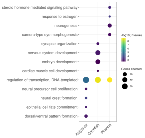
\includegraphics[width=1\textwidth]{Figures/astyanax/Go_acc_regions}
\caption[GO of ARs]{Dot plot illustrating the GO enrichment of the genes that are nearby CREs with ARs inside (putative enhancers with accelerated evolutionary rate). On the X-axis, species in which ARs have been computed. On the Y-axis are represented enriched GO terms. The dot size is proportional to the number of genes in the comparison corresponding to that GO term. The colour of the dots varies with the $-log10(PValue)$ of the enrichment. }
\label{fig:astmex_acc_regions_GO}
\end{figure}


